%%%%%%
% Author: Nikoloz Gochiashvili
% Resources from: http://www.joelonsoftware.com/articles/LeakyAbstractions.html
% CEN533 final

\documentclass{article}

% ------
% Fonts and typesetting settings
\usepackage[sc]{mathpazo}
\usepackage[T1]{fontenc}
\linespread{1.05} % Palatino needs more space between lines
\usepackage{microtype}
\usepackage[utf8]{inputenc}
\usepackage[english]{babel}
\usepackage{graphicx}

% ------
% Page layout
\usepackage[hmarginratio=1:1,top=32mm,columnsep=20pt]{geometry}
\usepackage[font=it]{caption}
\usepackage{paralist}
\usepackage{multicol}

% ------
% Lettrines
\usepackage{lettrine}


% ------
% Abstract
\usepackage{abstract}
	\renewcommand{\abstractnamefont}{\normalfont\bfseries}
	\renewcommand{\abstracttextfont}{\normalfont\small\itshape}


% ------
% Titling (section/subsection)
\usepackage{titlesec}
\renewcommand\thesection{\Roman{section}}
\titleformat{\section}[block]{\large\scshape\centering}{\thesection.}{1em}{}


% ------
% Header/footer
\usepackage{fancyhdr}
	\pagestyle{fancy}
	\fancyhead{}
	\fancyfoot{}
	\fancyhead[C]{nikoloz gochiashvili $\bullet$ February 2016 $\bullet$ The Law of Leaky Abstractions}
	\fancyfoot[RO,LE]{\thepage}


% ------
% Clickable URLs (optional)
\usepackage{hyperref}

% ------
% Maketitle metadata
\title{\vspace{-15mm}%
	\fontsize{24pt}{10pt}\selectfont
	\textbf{The Law of Leaky Abstractions}
	}	
\author{%
	\large
	\textsc{Nikoloz Gochiashvili} \\[2mm]
	\normalsize	International Black Sea University \\
	\normalsize	\href{mailto:ngochiashvili@gmail.com}{ngochiashvili@gmail.com}
	\vspace{-5mm}
	}
\date{}

\begin{document}

\maketitle
\thispagestyle{fancy}

\begin{abstract}
\noindent

\cite{JoelonAPIApology}All non-trivial abstractions, to some degree, are leaky."

This is overly dogmatic - for example, bignum classes are exactly the same regardless of the native integer multiplication. Ignoring that, this statement is essentially true, but rather inane and missing the point. Without abstractions, all our code would be completely interdependent and unmaintainable, and abstractions do a remarkable job of cleaning that up. It is a testament to the power of abstraction and how much we take it for granted that such a statement can be made at all, as if we always expected to be able to write large pieces of software in a maintainable manner.
\end{abstract}
	
\section{Introduction}

\lettrine[nindent=0em,lines=3]{T}here's a key piece of magic in the engineering of the Internet which you rely on every single day. It happens in the TCP protocol, one of the fundamental building blocks of the Internet.

TCP is a way to transmit data that is reliable. By this I mean: if you send a message over a network using TCP, it will arrive, and it won't be garbled or corrupted.

We use TCP for many things like fetching web pages and sending email. The reliability of TCP is why every exciting email from embezzling East Africans arrives in letter-perfect condition. O joy.

By comparison, there is another method of transmitting data called IP which is unreliable. Nobody promises that your data will arrive, and it might get messed up before it arrives. If you send a bunch of messages with IP, don't be surprised if only half of them arrive, and some of those are in a different order than the order in which they were sent, and some of them have been replaced by alternate messages, perhaps containing pictures of adorable baby orangutans, or more likely just a lot of unreadable garbage that looks like the subject line of Taiwanese spam.

Here's the magic part: TCP is built on top of IP. In other words, TCP is obliged to somehow send data reliably using only an unreliable tool.

To illustrate why this is magic, consider the following morally equivalent, though somewhat ludicrous, scenario from the real world.

Imagine that we had a way of sending actors from Broadway to Hollywood that involved putting them in cars and driving them across the country. Some of these cars crashed, killing the poor actors. Sometimes the actors got drunk on the way and shaved their heads or got nasal tattoos, thus becoming too ugly to work in Hollywood, and frequently the actors arrived in a different order than they had set out, because they all took different routes. Now imagine a new service called Hollywood Express, which delivered actors to Hollywood, guaranteeing that they would (a) arrive (b) in order (c) in perfect condition. The magic part is that Hollywood Express doesn't have any method of delivering the actors, other than the unreliable method of putting them in cars and driving them across the country. Hollywood Express works by checking that each actor arrives in perfect condition, and, if he doesn't, calling up the home office and requesting that the actor's identical twin be sent instead. If the actors arrive in the wrong order Hollywood Express rearranges them. If a large UFO on its way to Area 51 crashes on the highway in Nevada, rendering it impassable, all the actors that went that way are rerouted via Arizona and Hollywood Express doesn't even tell the movie directors in California what happened. To them, it just looks like the actors are arriving a little bit more slowly than usual, and they never even hear about the UFO crash.

That is, approximately, the magic of TCP. It is what computer scientists like to call an abstraction: a simplification of something much more complicated that is going on under the covers. As it turns out, a lot of computer programming consists of building abstractions. What is a string library? It's a way to pretend that computers can manipulate strings just as easily as they can manipulate numbers. What is a file system? It's a way to pretend that a hard drive isn't really a bunch of spinning magnetic platters that can store bits at certain locations, but rather a hierarchical system of folders-within-folders containing individual files that in turn consist of one or more strings of bytes.

Back to TCP. Earlier for the sake of simplicity I told a little fib, and some of you have steam coming out of your ears by now because this fib is driving you crazy. I said that TCP guarantees that your message will arrive. It doesn't, actually. If your pet snake has chewed through the network cable leading to your computer, and no IP packets can get through, then TCP can't do anything about it and your message doesn't arrive. If you were curt with the system administrators in your company and they punished you by plugging you into an overloaded hub, only some of your IP packets will get through, and TCP will work, but everything will be really slow.

\section{What I call a leaky abstraction}
 TCP attempts to provide a complete abstraction of an underlying unreliable network, but sometimes, the network leaks through the abstraction and you feel the things that the abstraction can't quite protect you from. This is but one example of what I've dubbed the Law of Leaky Abstractions:

"All non-trivial abstractions, to some degree, are leaky."

Abstractions fail. Sometimes a little, sometimes a lot. There's leakage. Things go wrong. It happens all over the place when you have abstractions. Here are some examples.

\begin{compactitem}
\item Something as simple as iterating over a large two-dimensional array can have radically different performance if you do it horizontally rather than vertically, depending on the "grain of the wood" -- one direction may result in vastly more page faults than the other direction, and page faults are slow. Even assembly programmers are supposed to be allowed to pretend that they have a big flat address space, but virtual memory means it's really just an abstraction, which leaks when there's a page fault and certain memory fetches take way more nanoseconds than other memory fetches.
\item The SQL language is meant to abstract away the procedural steps that are needed to query a database, instead allowing you to define merely what you want and let the database figure out the procedural steps to query it. But in some cases, certain SQL queries are thousands of times slower than other logically equivalent queries. A famous example of this is that some SQL servers are dramatically faster if you specify "where a=b and b=c and a=c" than if you only specify "where a=b and b=c" even though the result set is the same. You're not supposed to have to care about the procedure, only the specification. But sometimes the abstraction leaks and causes horrible performance and you have to break out the query plan analyzer and study what it did wrong, and figure out how to make your query run faster.
\item Even though network libraries like NFS and SMB let you treat files on remote machines "as if" they were local, sometimes the connection becomes very slow or goes down, and the file stops acting like it was local, and as a programmer you have to write code to deal with this. The abstraction of "remote file is the same as local file" leaks. Here's a concrete example for Unix sysadmins. If you put users' home directories on NFS-mounted drives (one abstraction), and your users create .forward files to forward all their email somewhere else (another abstraction), and the NFS server goes down while new email is arriving, the messages will not be forwarded because the .forward file will not be found. The leak in the abstraction actually caused a few messages to be dropped on the floor.
\item C++ string classes are supposed to let you pretend that strings are first-class data. They try to abstract away the fact that strings are hard and let you act as if they were as easy as integers. Almost all C++ string classes overload the + operator so you can write s + "bar" to concatenate. But you know what? No matter how hard they try, there is no C++ string class on Earth that will let you type "foo" + "bar", because string literals in C++ are always char*'s, never strings. The abstraction has sprung a leak that the language doesn't let you plug. (Amusingly, the history of the evolution of C++ over time can be described as a history of trying to plug the leaks in the string abstraction. Why they couldn't just add a native string class to the language itself eludes me at the moment.)
\item And you can't drive as fast when it's raining, even though your car has windshield wipers and headlights and a roof and a heater, all of which protect you from caring about the fact that it's raining (they abstract away the weather), but lo, you have to worry about hydroplaning (or aquaplaning in England) and sometimes the rain is so strong you can't see very far ahead so you go slower in the rain, because the weather can never be completely abstracted away, because of the law of leaky abstractions.
\end{compactitem}

\section{Abstraction problem}

One reason the law of leaky abstractions is problematic is that it means that abstractions do not really simplify our lives as much as they were meant to. When I'm training someone to be a C++ programmer, it would be nice if I never had to teach them about char*'s and pointer arithmetic. It would be nice if I could go straight to STL strings. But one day they'll write the code "foo" + "bar", and truly bizarre things will happen, and then I'll have to stop and teach them all about char*'s anyway. Or one day they'll be trying to call a Windows API function that is documented as having an OUT LPTSTR argument and they won't be able to understand how to call it until they learn about char*'s, and pointers, and Unicode, and wchar\_t's, and the TCHAR header files, and all that stuff that leaks up.

In teaching someone about COM programming, it would be nice if I could just teach them how to use the Visual Studio wizards and all the code generation features, but if anything goes wrong, they will not have the vaguest idea what happened or how to debug it and recover from it. I'm going to have to teach them all about IUnknown and CLSIDs and ProgIDS and ... oh, the humanity!

In teaching someone about ASP.NET programming, it would be nice if I could just teach them that they can double-click on things and then write code that runs on the server when the user clicks on those things. Indeed ASP.NET abstracts away the difference between writing the HTML code to handle clicking on a hyperlink (<a>) and the code to handle clicking on a button. Problem: the ASP.NET designers needed to hide the fact that in HTML, there's no way to submit a form from a hyperlink. They do this by generating a few lines of JavaScript and attaching an onclick handler to the hyperlink. The abstraction leaks, though. If the end-user has JavaScript disabled, the ASP.NET application doesn't work correctly, and if the programmer doesn't understand what ASP.NET was abstracting away, they simply won't have any clue what is wrong.

The law of leaky abstractions means that whenever somebody comes up with a wizzy new code-generation tool that is supposed to make us all ever-so-efficient, you hear a lot of people saying "learn how to do it manually first, then use the wizzy tool to save time." Code generation tools which pretend to abstract out something, like all abstractions, leak, and the only way to deal with the leaks competently is to learn about how the abstractions work and what they are abstracting. So the abstractions save us time working, but they don't save us time learning.

And all this means that paradoxically, even as we have higher and higher level programming tools with better and better abstractions, becoming a proficient programmer is getting harder and harder.

During my first Microsoft internship, I wrote string libraries to run on the Macintosh. A typical assignment: write a version of strcat that returns a pointer to the end of the new string. A few lines of C code. Everything I did was right from K\&R -- one thin book about the C programming language.

Today, to work on CityDesk, I need to know Visual Basic, COM, ATL, C++, InnoSetup, Internet Explorer internals, regular expressions, DOM, HTML, CSS, and XML. All high level tools compared to the old K\&R stuff, but I still have to know the K\&R stuff or I'm toast.

Ten years ago, we might have imagined that new programming paradigms would have made programming easier by now. Indeed, the abstractions we've created over the years do allow us to deal with new orders of complexity in software development that we didn't have to deal with ten or fifteen years ago, like GUI programming and network programming. And while these great tools, like modern OO forms-based languages, let us get a lot of work done incredibly quickly, suddenly one day we need to figure out a problem where the abstraction leaked, and it takes 2 weeks. And when you need to hire a programmer to do mostly VB programming, it's not good enough to hire a VB programmer, because they will get completely stuck in tar every time the VB abstraction leaks.

The Law of Leaky Abstractions is dragging us down.

\centering
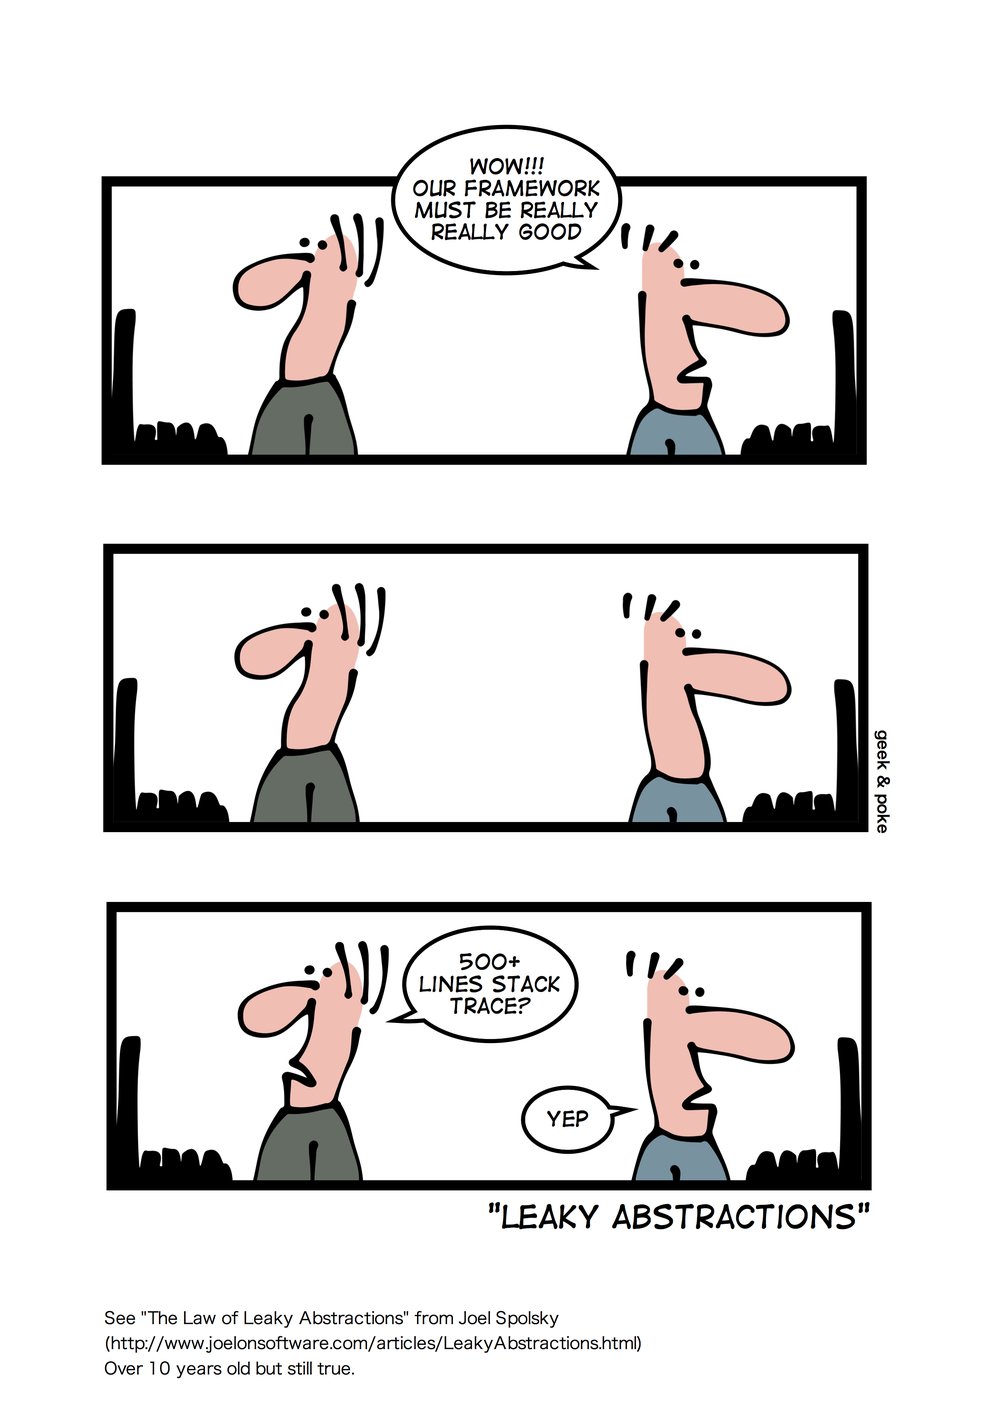
\includegraphics{good-framework.jpg}

\bibliography{bibliography}{}
\bibliographystyle{plain}

\end{document}
